% \documentclass[pdfCover]{myreport} % 需要pdf封面
\documentclass{myreport}
\title{图像分割与边缘检测}
\author{陈伯硕}
\date{\today}

\def\MyProject{数字图像处理}

\fancyhead{} % Clear the headers
\renewcommand{\headrulewidth}{1pt} % Width of line at top of page
\fancyhead[L]{\MyProject}
\fancyhead[R]{\MyTitle} % Mark right [R] of page with Chapter name [\leftmark]


\usepackage{subfiles}
\begin{document}

\maketitle

\section{边缘检测}
  \subsection{Sobel}
      % \cref{fig:fish}
      \begin{figure}[H]
        \centering
        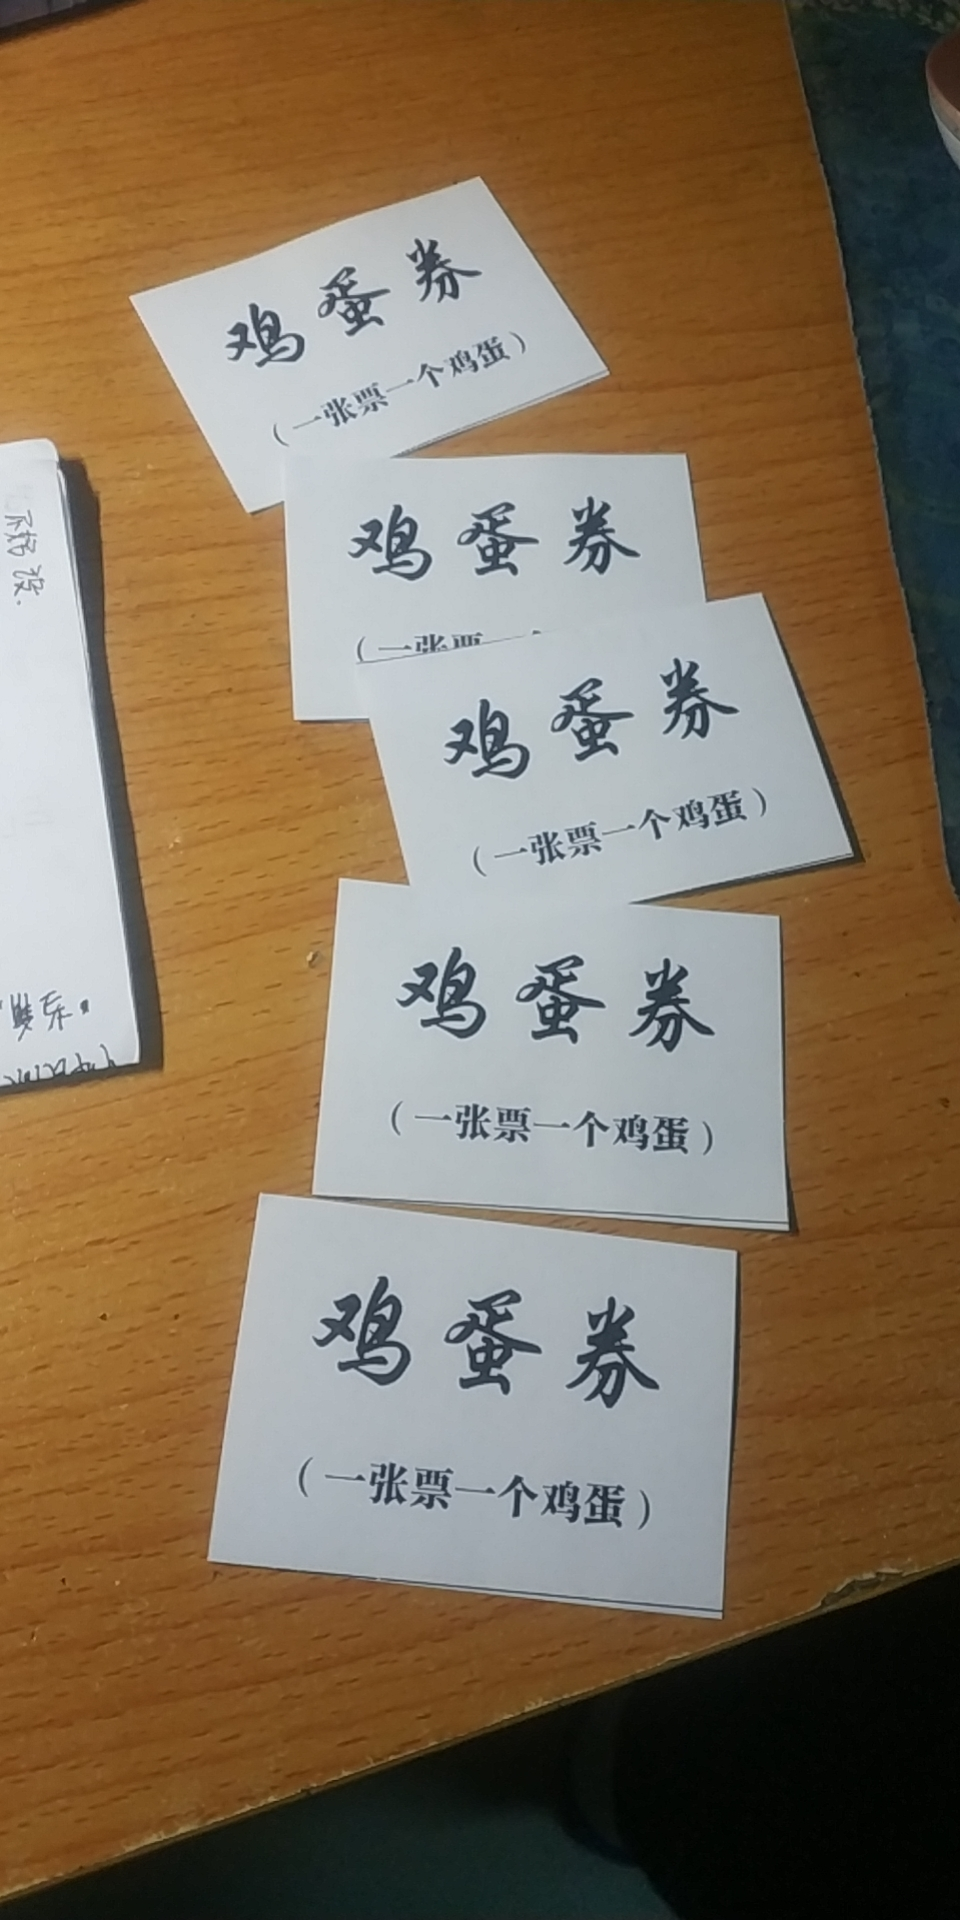
\includegraphics[width = 0.6\textwidth]{raw}
        \caption{图片来自 Bing 2022-11-14 封面图}
        \label{fig:fish}
      \end{figure}

      设$A$为原图像,则sobel滤波可表示为
      $$
        G_x = \begin{bmatrix}
            -1 & 0 & 1 \\
            -2 & 0 & 2 \\
            -1 & 0 & 1
        \end{bmatrix}
        \circledast A 
      $$
      
      $$
        G_y = \begin{bmatrix}
            1 & 2 & 1 \\
            0 & 0 & 0 \\
            -1 & -2 & -1
        \end{bmatrix}
        \circledast A 
      $$
      
      $$
        A'(x,y) = |G'_x(x,y)| + |G'_y(x,y)| 
      $$

      % \cref{fig:sobel}
      \begin{figure}[H]
        \centering
        \includegraphics[width = \textwidth]{sobel}
        \caption{依次为$G_x, G_y, A'$和skimagee.fiter.sobel的结果}
        \label{fig:sobel}
      \end{figure}

  \subsection{prewitt}
      $$
        G'_x = \begin{bmatrix}
            -1 & 0 & 1 \\
            -1 & 0 & 1 \\
            -1 & 0 & 1
        \end{bmatrix}
        \circledast A 
      $$
      
      $$
        G'_y = \begin{bmatrix}
            1 & 1 & 1 \\
            0 & 0 & 0 \\
            -1 & -1 & -1
        \end{bmatrix}
        \circledast A 
      $$
      
      $$
        A''(x,y) = |G'_x(x,y)| + |G'_y(x,y)| 
      $$

      % \cref{fig:sobel_compare}
      \begin{figure}[H]
        \centering
        \includegraphics[width = \textwidth]{sobel_vs_prewitt}
        \caption{$A',A''$结果对比}
        \label{fig:sobel_compare}
      \end{figure}
      两者整体上差别不大,Sobel算子的图灰度相差似乎更明显
      % \cref{fig:sobel_compare}
      \begin{figure}[H]
        \centering
        \includegraphics[width = 0.6\textwidth]{sobel_compare}
        \caption{两者的灰度分布}
        \label{fig:sobel_compare}
      \end{figure}
   
      % \cref{fig:diff}
      \begin{figure}[H]
        \centering
        \includegraphics[width = \textwidth]{diff}
        \caption{sobel VS perwitt}
        \label{fig:diff}
      \end{figure}
      竖直方向有细微差别,
      可能由于perwitt是上下差分,
      sobel将像素点上下邻居加强导致

\section{Hough 线检测}
  通常,直线被参数化为 $y = mx + c$,
  有一个梯度 $m$ 和 $y$ 截距 $c$。
  然而,这意味着对于垂直直线,
  $m$ 趋向于无穷大。
  因此,我们构造一个垂直于直线的线段,通向原点。
  这条直线用这段的长度 $r$ 和它与 $x$ 轴的夹角 $\theta$ 
  来表示。
  Hough 变换构造了一个表示参数空间的直方图数组
  (即 $M \times N$ 矩阵,
  对于 $M$ 个不同的半径值和 $N$ 个不同的 $\theta$ 值)。
  对于每个参数组合 $r$ 和 $\theta$,
  然后我们找到输入图像中接近对应直线的非零像素数,
  并适当地增加数组的位置$(r,\theta)$。
  我们可以考虑每个非零像素“投票”的潜在线候选人。
  结果直方图中的局部极大值表示最可能的直线的参数。
  在我们的例子中,
  最大值出现在45度和135度,
  对应于每条直线的法向量角。
  另一种方法是渐进概率 Hough 变换。
  该算法基于这样一个假设,
  即使用随机的投票点子集,
  也能很好地逼近实际结果,
  并且在投票过程中可以通过沿连通分量行走来提取直线。
  这将返回每个行段的开始和结束,这很有用。
  函数概率霍夫有三个参数: 
  一个应用于霍夫累加器的通用阈值,
  一个最小线长度和影响线合并的线间隙。
  在下面的示例中,我们发现行长大于10,间隔小于3像素。
  \begin{figure}[H]
    \centering
    \includegraphics[width = 0.6\textwidth]{hough_example}
    \caption{Hough 线 example}
    \label{fig:hough}
  \end{figure}

  % \cref{fig:hough}
  \begin{figure}[H]
    \centering
    \includegraphics[width = 0.6\textwidth]{hough}
    \caption{Hough 线检测}
    \label{fig:hough}
  \end{figure}
  python 的hough线检测是使用的原始定义,
  官方文档为简单的三条线,
  找到了交点,而样例图片边框复杂,没有太好的效果
  


  % \cref{fig:probabilistic_hough}
  \begin{figure}[H]
    \centering
    \includegraphics[width = 0.6\textwidth]{probabilistic_hough}
    \caption{skimage 推荐的 probabilistic hough 方法找边界}
    \label{fig:probabilistic_hough}
  \end{figure}
\section{图像二值分割}

  % \cref{fig:threshold}
  \begin{figure}[H]
    \centering
    \includegraphics[width = 0.6\textwidth]{threshold}
    \caption{实例图像的阈值}
    \label{fig:threshold}
  \end{figure}

  % \cref{fig:bin}
  \begin{figure}[H]
    \centering
    \includegraphics[width = 0.6\textwidth]{bin}
    \caption{二值分割后的结果}
    \label{fig:bin}
  \end{figure}

\begin{appendices} % 附录
  \includepdf[pages={1},pagecommand=\section*{源代码}]{attachment/build/image_processing.pdf}
  \includepdf[pages={2-},pagecommand=\section*{\quad}]{attachment/build/image_processing.pdf}

\end{appendices}
\end{document}
